\documentclass[titlepage]{scrartcl}
\usepackage{graphicx}
\usepackage{float}
\usepackage[]{biblatex}
\usepackage{textgreek}
\addbibresource{bibliography.bib}
\addtokomafont{disposition}{\rmfamily}
%opening
\titlehead{BIOL 224L}
\title{Assignment 2}
\date{\today}
\author{Dean Pearce}

\begin{document}

\maketitle
\section{Problem 1}
The original stoichiometry is broadly, uniquely interesting.  Broadly, the $1A+2B \rightarrow 3B$ system is the most agile proof of the concept of irreversible conversion of a field of A to B.  Altering the formula to $1A+3B \rightarrow 4B$ does not add any novel utility of its own, but rather results in a rather uninteresting slow spread of B conversion.
\section{Problem 2}
The Gray-Scott model is broadly unsensitive to initial conditions.  The novelty of the behavior is enshrined in the stoichiometry and the parameters, the initial conditions are largely irrevelant.  Even when the initial conditions are altered dramatically, the overall product looks similar in concept.
\section{Problem 3}
A particularly volatile region in parameter space is as shown.
\begin{figure}[H]
    \centering
    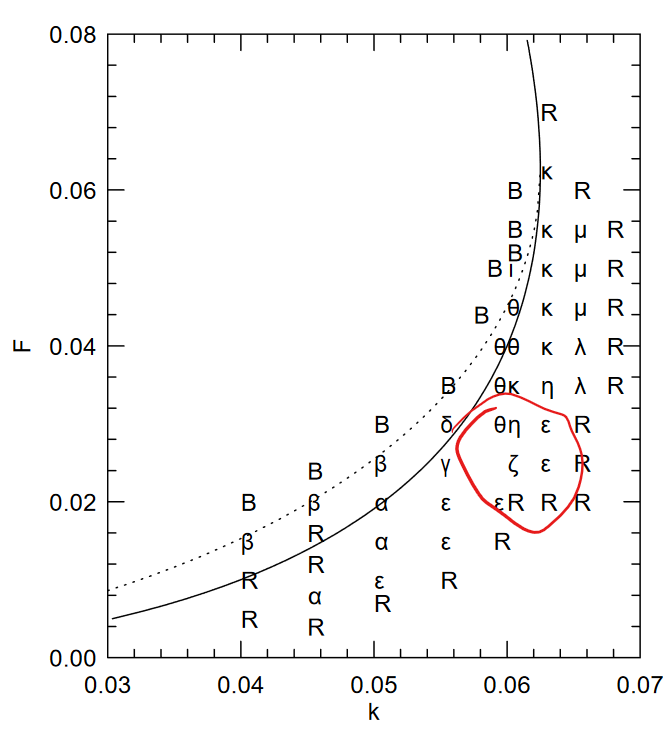
\includegraphics[scale=0.5]{graph.png}
\end{figure}
Broadly speaking, the established method to characterize Gray-Scott systems is with Pearson's Typology\cite{pearsonComplexPatternsSimple1993}, which utilizes a number of symbols, the same depicted in the graph, and is  is described as follows.
\subsection{Pearson's Typology}
\begin{description}
    \item[R] Uniform red state at stability
    \item[\textalpha] "fledgling spirals which are constantly colliding and annihilating each other"
    \item[\textbeta] "phase turbulence", highly chaotic
    \item[\textgamma] primarily of stripes with localized oscillations
    \item[\textsigma] hexagons
    \item[\texteta] stripes with oscillations
    \item[\textiota]  disordered circles
    \item[\textmu] long stripes
    \item[\texttheta, \textkappa] Broadly similar, form "mazes" radiating outward from B deposit; \texttheta has a more complex "maze"
    \item[\textlambda] many dots, which split until the cover the field and are relatively evenly spaced
    \item[\textepsilon] similar to \texttheta, but occassionally the "dots" will dissappear, and a nearby dot split to take its space.
    \item[\textzeta] dots also cover the field, with localized pulsations; occassionally the dots at the center of pulsation will dissappear, and the surroundings move to fill the gap.
    \item[B] Uniform blue state at stability
\end{description}
\begin{figure}[h]
    \centering
    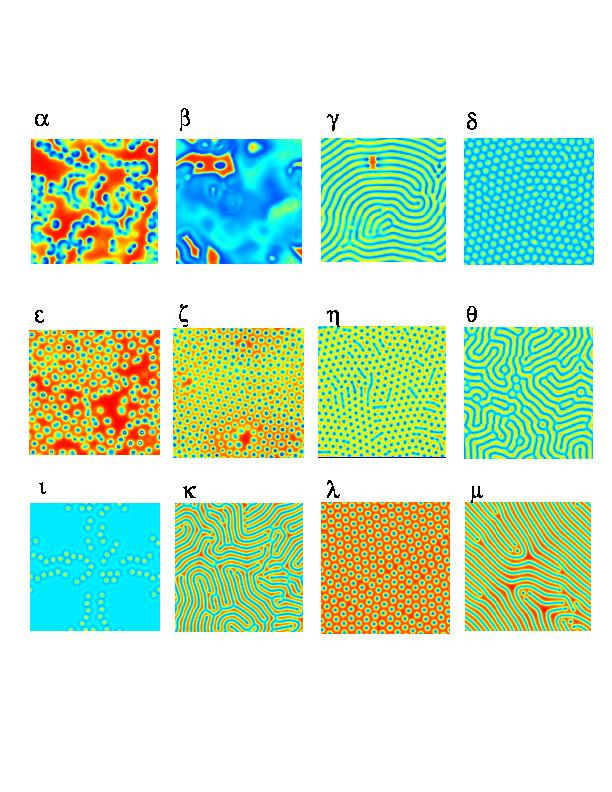
\includegraphics[scale=0.5]{fig2.jpg}
    \caption[Pearson's Typology Key]{Illustrations of Pearson's Typologies}
\end{figure}
\printbibliography
\end{document}
